\chapter{Despacho de Energia}
O conjunto de vari\'aveis que identificam o desenvolvido de um pa\'is \'e extremamente complexo. Uma das vari\'aveis
utilizadas nessa
an\'alise \'e a facilidade que a popula\c c\~ao tem acesso a estrutura b\'asica de servi\c cos como: saneamento
b\'asico, transportes, as telecomunica\c c\~oes e a energia \cite{an}. Essa \'ultima recebe uma aten\c c\~ao especial,
por ser 
indispens\'avel para as atividades humanas que necessitam de um algum tipo de maquin\'ario. No planejamento energ\'etico de uma na\c
c\~ao dois aspectos necessitam est\'a bem definidos, os quais s\~ao : a matriz energ\'etica e a matriz el\'etrica. A matriz
energ\'etica \'e definida como todas as fontes de energia dispon\'iveis para o funcionamento de alguma tecnologia
humana. Enquanto, a matriz el\'etrica \'e definida como todas as fontes de energia dispon\'ivies para a gera\c c\~ao
el\'etrica. Primeiramente, ser\'a considerado a an\'alise de um aspecto geral, ou seja, a matriz energ\'etica. O
 setor energ\'etico brasileiro historicamente \'e constitu\'ido por duas situa\c c\~oes extremas na an\'alise da matriz
 energ\'etica. 

A primeira situa\c c\~ao tem rela\c c\~ao
com o desenvolvimento tecnol\'ogico, particularmente a efici\^encia energ\'etica. O intuito da efici\^encia energ\'etica
\'e o desenvolvimento de novas tecnologias que utilizem de forma satisfat\'oria a energia dispon\'ivel, al\'em de 
otimizar as t\'ecnicas para a produ\c c\~ao energ\'etica. Para exemplificar o primeiro ponto pode-se
considerar o caso do autom\'ovel que por muitas d\'ecadas empregava como a sua principal fonte de energia a gasolina,
por\'em gradualmente sua fonte de energia est\'a sendo modificada para atender outras formas de combust\'ivel como o
etanol \cite{an}. Com a rela\c c\~ao ao segundo ponto, na atualidade o principal destaque deve-se as pesquisas por novas
fontes de energia como: geot\'ermica, c\'elulas de hidrog\^enio, e\'olica e solar.

A segunda situa\c c\~ao tem como objetivo
garantir que a popula\c c\~ao tenha acesso as novas tecnologias de maneira
simples, eficaz e de baixo custo. O principal reflexo dessa iniciativa \'e observado no fornecimento de energia
el\'etrica \cite{an}. Contudo, sua influ\^encia tamb\'em \'e percebida em outros setores em uma menor escala. Por
exemplo, na d\'ecada de 70 a substitui\c c\~ao da lenha por derivados do petr\'oleo (GLP-g\'as liquefeito do
petr\'oleo) ocasinou uma mudan\c ca significativa no modo de vida da popula\c c\~ao, pois permitiu uma maior efici\^encia na
produ\c c\~ao aliment\'icia brasileira \cite{an}. Essa situa\c c\~ao exemplificar como a matriz en\'ergetica \'e
constitu\'ida de outros setores,
al\'em do el\'etrico em sua constru\c c\~ao. A \fig{comparation} a seguir traz um comparativo com as principais diferen\c cas entre a matriz
energ\'etica brasileira e a matriz mundial.
\begin{figure}[!h]
	\centering
	\subfigure[Matriz energ\'etica mundial]{
		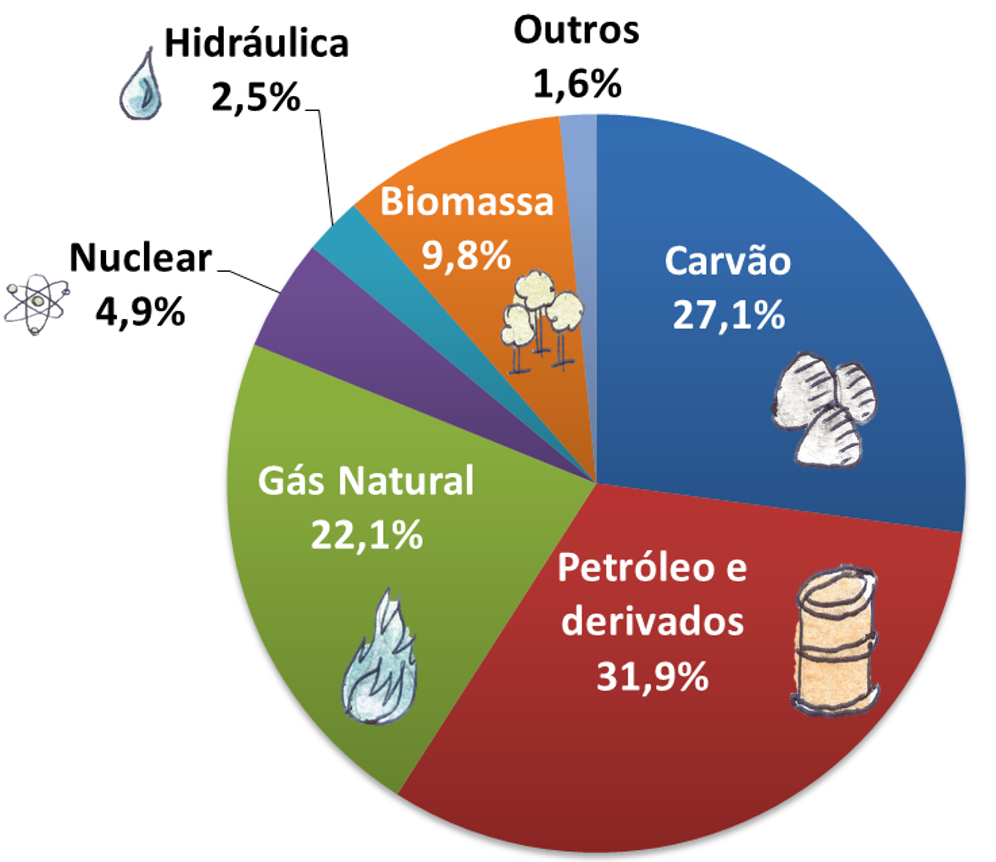
\includegraphics[width=7cm]{material/mundo.png}
	}
	\quad \quad
	\subfigure[Matriz energ\'etica brasileira]{
		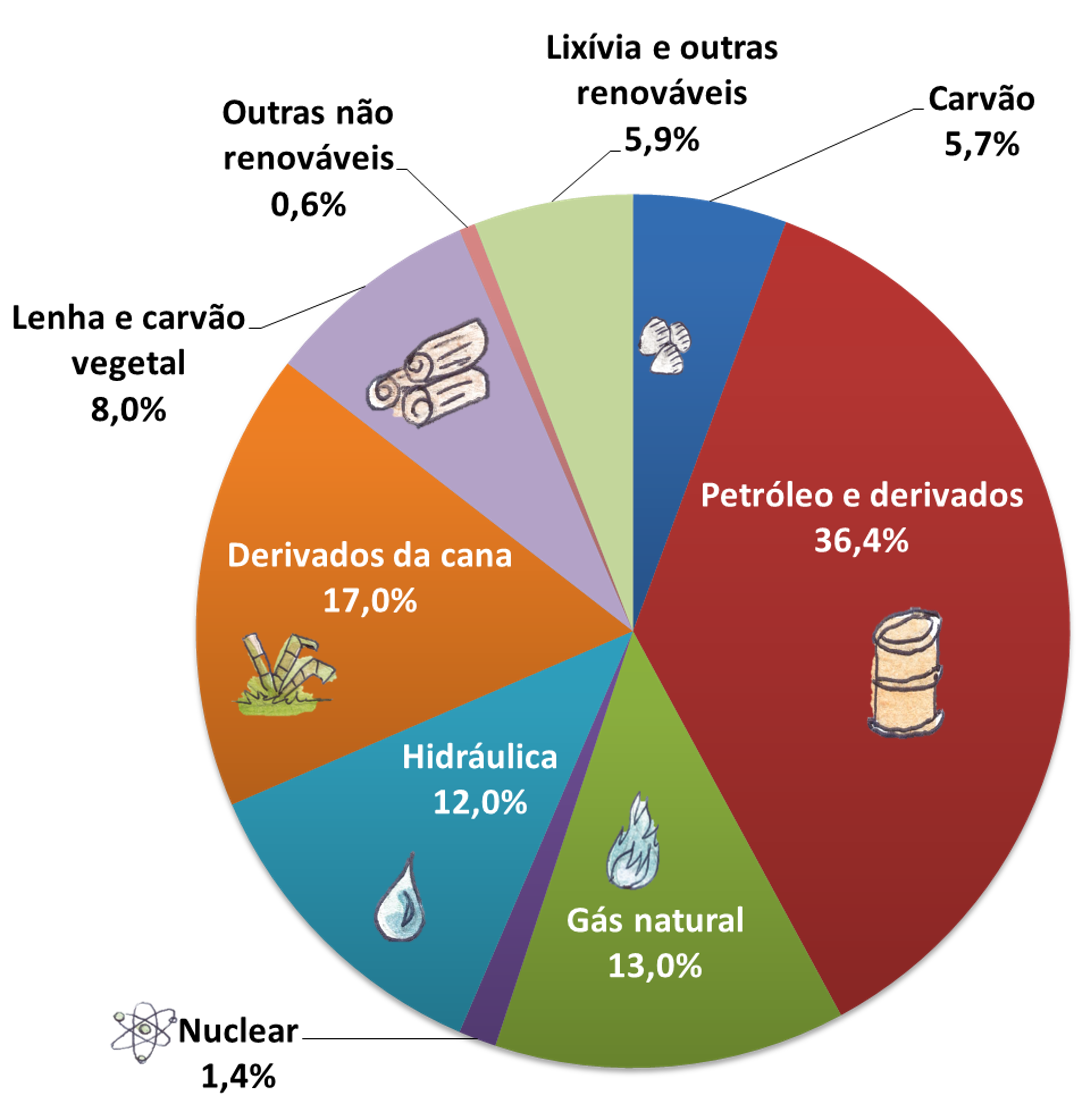
\includegraphics[width=6.5cm]{material/brasil.png}
	}
	\caption[A matriz energ\'etica mundial e a brasileira.]{A matriz energ\'etica mundial e a brasileira.}{Fonte: Empresa de Pesquisa Energ\'etica.}
	\label{comparation}
\end{figure}

Nota-se que pela \fig{comparation}(a) que matriz energ\'etica mundial \'e constitu\'ida principalmente por fontes n\~ao
renov\'aveis. Contudo, ao contr\'ario do cen\'ario mundial no Brasil h\'a uma grande utiliza\c c\~ao de energias
renov\'aveis, como ilustra a \fig{comparation}(b) destacando-se a gera\c c\~ao el\'etrica do tipo energia
hidr\'aulica.

Uma vez que os aspectos referentes a matriz en\'ergetica foram retratados. Para o presente trabalho ser\'a considerado
somente a matriz el\'etrica brasileira com rela\c c\~ao a eletricidade, isto \'e, a matriz el\'etrica. Dentre todos
os segmentos de infra-estrutura o de energia \'e o que possui uma maior abrang\^encia \cite{an}. O sistema
energ\'etico brasileiro abrange um consider\'avel conjunto de nichos. Contudo, h\'a uma quantidade de nichos que
constituem uma dificuldade para o sistema. A incid\^encia e as dimens\~oes dos nichos\footnote {Nicho \'e o termo utilizado para
definir determinado p\'ublico ou setor com caracter\'isticas especificas ou particulares a serem atendidas.} n\~ao atendidos est\~ao diretamente
relacionada a fatores como a localiza\c c\~ao e as dificuldades f\'isicas ou econ\^omicas para a expans\~ao da rede
el\'etrica \cite{an}. Essas dificuldades devem-se pelo Brasil ser constitu\'ido por cinco regi\~oes geogr\'aficas: Sul,
Sudeste, Norte, Nordeste, Centro-Oeste. Cada uma das regi\~oes mencionadas possui suas caracter\'isticas particulares
como: relevo, hidrografia e economia. Esses fatores interferem de forma substancial no abastecimento. Uma vez
que tais caracter\'isticas determinam os contornos que a configura\c c\~ao do sistema de gera\c c\~ao e transmiss\~ao devem 
obedecer\cite{an}. Portanto, as caracter\'isticas regionais indicam como a popula\c c\~ao tem acesso a energia
el\'etrica. No caso do Brasil o sistema el\'etrico \'e constitu\'ido por tr\^es grande blocos que constituem o sistema
el\'etrico nacional: Gera\c c\~ao, Transmiss\~ao e Distribui\c c\~ao. A \fig{energia} a seguir exemplificar os processos
mencionados no sistema el\'etrico nacional.

\begin{figure}[!h]
	\centering
	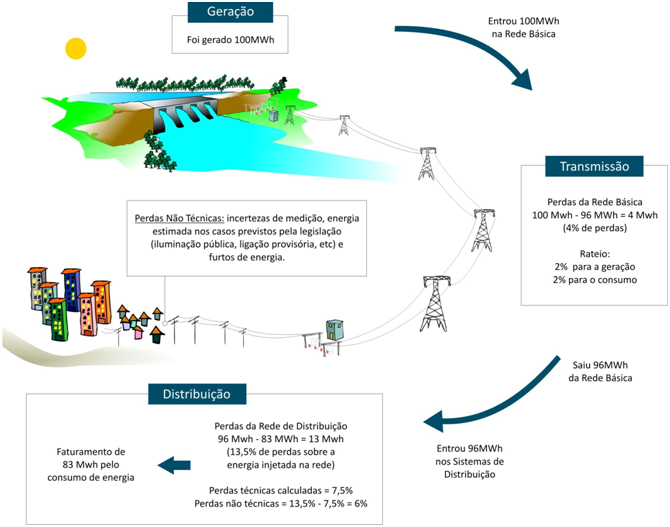
\includegraphics[width=11cm]{material/perdas.jpg}
	\caption[Gera\c c\~ao, Transmiss\~ao e Distribui\c c\~ao. ]{Gera\c c\~ao, Transmiss\~ao e Distribui\c c\~ao.}{Fonte: Ag\^encia Nacional de Energia El\'etrica.}
	\label{energia} 
\end{figure}

No gerenciamento e transmiss\~ao da energia el\'etrica, o Brasil possui o Sistema Interligado Nacional (SIN)
eerenciado pelo Operador Nacional de Energia (ONS)
 correspondendo as regi\~oes Sul, Sudeste, Centro-Oeste, Nordeste e parte do Norte. O SIN \'e respons\'avel por abrigar cerca de
$96,6\%$ de toda a capacidade de produ\c c\~ao de energia do Brasil, seja por meio de fontes internas de energia
ou pela importa\c c\~ao de energia como ocorre na usina de Itaipu mediante o controle compartilhado com o
Paraguai\cite{an}. A ado\c c\~ao do SIN \'e justificada tendo por base: o interc\^ambio energ\'etico, a
complementaridade entre fontes de gera\c c\~ao de energia e pela sua capacidade de expans\~ao.

O interc\^ambio energ\'etico permite que regi\~oes que estejam vinculada ao SIN possam auxiliar no suprimento da
demanda de outras de regi\~oes que por algum fator interno ou externo n\~ao conseguem manter a demanda na sua localidade\cite{an}. Por
exemplo, considerando-se que determinadas regi\~oes brasileiras podem sofrer com a escassez de chuva o que implica na
baixa pluviosidade. Essa regi\~ao corre o risco de enfrentar problemas de abastecimento caso sua fonte de gera\c c\~ao
de energia el\'etrica seja por meio de hidrel\'etricas. Nesse tipo de situa\c c\~ao \'e totalmente poss\'ivel que outra
regi\~ao que n\~ao esteja enfrentando problemas de escassez auxiliar enviando energia el\'etrica para atender a
localidade que esteja enfretando problemas de abastecimento. 

A complementaridade entre fontes de energia tem o mesmo princ\'ipio do interc\^ambio, contudo seu principal objetivo \'e permitir
que uma ou mais regi\c c\~oes sejam abastecidas por diferente tipos de fonte de energia no intuito do sistema funcionar
da melhor forma poss\'ivel \cite{an}. Isto \'e, localizadades que possuem como sua principal fonte de energia a
hidrel\'etrica podem sofrer com o baixos \'indices de seus reservat\'orios. Nesse tipo de situa\c c\~ao
\'e comum a ativa\c c\~ao de termel\'etricas para auxiliar o abastecimento. Esse \'e um exemplo t\'ipico de
complementaridade oferecido pelo SIN. 

Uma vez que a energia el\'etrica gerada pela hidrel\'etrica possui um custo menor
que a mesma quantidade de energia el\'etrica produzida por uma termel\'etrica, portanto, deve-se manter como meta a utiliza\c c\~ao
da hidrel\'etrica para diminui poss\'iveis custos ao consumido\cite{an}. Contudo, apesar da termel\'etrica possui um
custo maior para a gera\c c\~ao de energia essa n\~ao possui o problema de abastecimento da hidrel\'etrica.
Portanto, a complementaridade para este caso seria configurar a utiliza\c c\~ao da hidrel\'etrica para a maioria dos
casos e a ativa\c c\~ao da termel\'etrica para auxiliar caso houvesse um pico de demanda ou problemas de
abastecimento por fatores como a pluviosidade.  

A expans\~ao \'e caracterizada por permitir que o SIN ao longo do tempo tenha condi\c c\~oes de assimilar outras hidrel\'etricas ou
regi\~oes permitindo que o sistema possua condi\c c\~oes de garantir a demanda mesmo com o aumento do consumo ou
poss\'iveis problemas de abastecimento por outros fatores internos ou externos. Por exemplo, em 2003 o SIN possuia 77,6
mil quil\^ometros de rede no per\'iodo de 2008 sua extens\~ao era 89,2 mil quil\^ometros de rede \cite{an}. 

O custo associado a produ\c c\~ao de energia \'e uma das vari\'aveis que influ\^encia o pre\c co. Na an\'alise do
sistema o pre\c co varia conforme o tipo de energia utilizada \cite{an}. Desta forma, o planejamento energ\'etico
depende do custo de produ\c c\~ao para determinar o despacho de energia. O despacho de energia \'e definido como quais
usinas devem ser mantidas ativas e quais precisam ser desativadas tomando-se em considera\c c\~ao a demanda, a oferta e
o custo de produ\c c\~ao do sistema.

Na an\'alise do custo de produ\c c\~ao para o despacho de energia outro fator a ser considerado s\~ao os sistemas
isolados. Os sistemas isolados est\~ao localizados principalmente na regi\~ao Norte,
estados como Amazonas, Roraima, Acre, Amap\'a e Rond\^onia. Esta denomina\c c\~ao deve-se por n\~ao estarem interligados ao
SIN e por n\~ao permitirem um interc\^ambio com outras regi\~oes devido as caracter\'istricas geogr\'aficas. O
funcionamento dos sistemas isolados \'e predominantemente t\'ermico. Os custos para a gera\c c\~ao de energia nesses sistemas s\~ao
superiores ao SIN por serem predominantemente t\'ermicos e pela sua localiza\c c\~ao requerer alto custo no
transporte de combust\'iveis \cite{an}. Como alternativa para o barateamento da energia gerada pelos sistemas isolados
foi constitu\'ido imposto denominado Conta de Consumo de Combust\'iveis (CCC) que permite subs\'idiar a compra de
combust\'ivies garantindo que popula\c c\~ao dessas localidades tenha alguns dos benef\'icios do SIN. 

A produ\c c\~ao de eletricidade no sistema brasileiro tem como objetivo principal minimizar
os custo de opera\c c\~ao e garantir o suprimento de energia em todo o pa\'is \cite{tom}. Devido ao SIN ser
constitu\'ido predominantemente por um sistema hidrot\'ermico(hidrel\'etricas e termel\'etricas em regime de
complementaridade) este \'e afetado pela incerteza associada a pluviosidade
das regi\~oes que o constituem\cite{an}. Al\'em da pluviosidade o sistema hidrot\'ermico brasileiro \'e constitu\'ido
pelas seguinte caracter\'isticas:
\begin{itemize}
	\item \textit{Sazonalidade intra natural}. Al\'em da variabilidade natural ocorre um varia\c c\~ao entre as esta\c
		c\~oes do ano. 
	\item \textit{A complementariedade e diversidade regional}. As bacias brasileiras possuem caracter\'isticas
		f\'isicas e clim\'aticas distintas. Outro ponto a ser observado \'e que no momento que ocorre um estiagem no
		Nordeste as bacias do Sul podem est\'a com um alto n\'ivel dos reservat\'orios dada a pluviosidade da regi\~ao,
		ou seja, h\'a uma complementariedade entre as regi\~oes do Brasil.
	\item \textit{O acoplamento espacial}. Na forma de cascata as usinas que est\~ao mais perto da jusante possuem depend\^encia
		de usinas mais perto da montante.
	\item \textit{O acoplamento temporal}. Na forma de cascata decis\~oes sobre a utiliza\c c\~ao possuem
		consequ\^encias no futuro. 
	\item \textit{Custo term\'eletrico}. Usinas term\'eletricas possuem um custo alto de produ\c c\~ao el\'etrica em
		rela\c c\~ao as hidrel\'etricas.
	\item \textit{Aspecto ambiental}. Usinas termel\'etricas possuem um alto impacto ambiental.
\end{itemize}

As caracterist\'icas mencionadas caracterizam o problema de despacho de energia hidrot\'ermico. A \fig{st}  exemplificar
o acoplamento temporal e espacial entre as usinas em cascata.
\begin{figure}[!htpb]
  \centering
  \resizebox{0.7\textwidth}{!}{%
  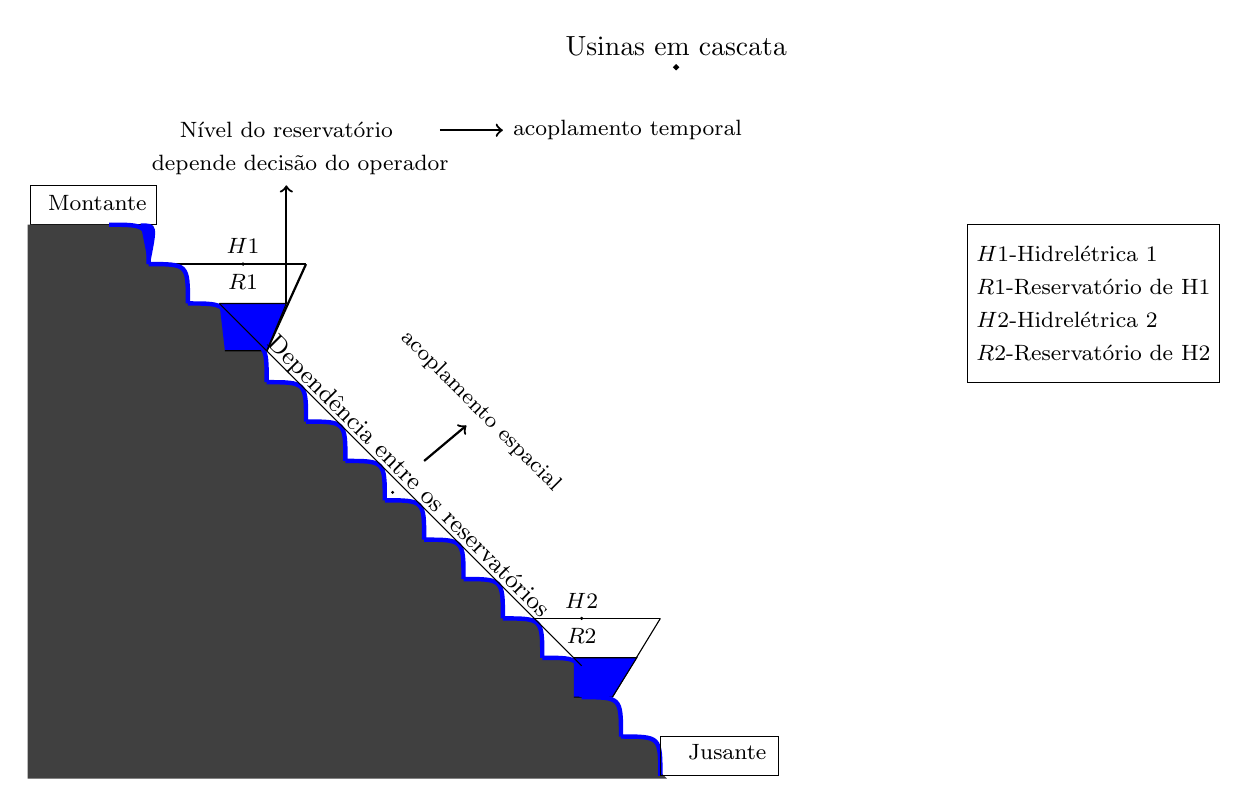
\begin{tikzpicture}
  % Desenho da cascata
  \draw [ultra thick,black] (7.2,9.0) circle (0.01mm) node[above]{Usinas em cascata};
  %
  % Desenho da montante
  \draw (-1.0,7.0) rectangle (0.6, 7.5) 
  node[below left] {\footnotesize Montante};
  %
  % Desenho da jusante

  \draw [thick, black]  (-1,0)--(-1,7);
  \draw [thick, black]  (-1,0)--(7,0);
  \draw [fill=darkgray] (-1.0,7.0) .. controls (0.5,7.0) .. (0.5,6.5);
  \draw [fill=darkgray] (0.0,7.0) .. controls (0.5,7.0) .. (0.5,6.5);
  \draw [fill=darkgray] (0.5,6.5) .. controls (1.0,6.5) .. (1.0,6.0);
  \draw [fill=darkgray] (1.0,6.0) .. controls (1.5,6.0) .. (1.5,5.5);
  \draw [fill=darkgray] (1.5,5.5) .. controls (2.0,5.5) .. (2.0,5.0);
  \draw [fill=darkgray] (2.0,5.0) .. controls (2.5,5.0) .. (2.5,4.5);
  \draw [fill=darkgray] (2.5,4.5) .. controls (3.0,4.5) .. (3.0,4.0);
  \draw [fill=darkgray] (3.0,4.0) .. controls (3.5,4.0) .. (3.5,3.5);
  \draw [fill=darkgray] (3.5,3.5) .. controls (4.0,3.5) .. (4.0,3.0);
  \draw [fill=darkgray] (4.0,3.0) .. controls (4.5,3.0) .. (4.5,2.5);
  \draw [fill=darkgray] (4.5,2.5) .. controls (5.0,2.5) .. (5.0,2.0);
  \draw [fill=darkgray] (5.0,2.0) .. controls (5.5,2.0) .. (5.5,1.5);
  \draw [fill=darkgray] (5.5,1.5) .. controls (6.0,1.5) .. (6.0,1.0);
  \draw [fill=darkgray] (6.0,1.0) .. controls (6.5,1.0) .. (6.5,0.5);
  \draw [fill=darkgray] (6.5,0.5) .. controls (7.0,0.5) .. (7.0,0.0);
  \draw [fill=darkgray,line width=0.1pt, opacity=100] (0,7)--(7,0);
  \filldraw [darkgray, line width=2.0pt] (0,7)--(7,0)--(-1,0)--(-1,7);
  %
  % Desenho de H1 
  \draw [thick, black] (1.7,6.5) circle (0.01mm) node [above]{\footnotesize $H1$};
  \draw [thick, black] (0.5,6.5)--(2.5,6.5);
  \draw [thick, black] (1.7,6.5) circle (0.01mm) node [below]{\footnotesize $R1$};
  \draw [thick, black] (2.5,6.5)--(2.0,5.4);
  
  \draw [fill=blue](1.40,6.0)--(2.25,6.0)--(2.0,5.4)--(1.47,5.4);
  % 
  % Desenho de H2
  \draw [thick, black] (6.0, 2.0) circle (0.01mm) node[above]{ \footnotesize $H2$};
  \draw [fill=darkgray] (5.0,2.0) -- (7.0,2.0);
  \draw [thick, black] (6.0,2.0) circle (0.01mm) node [below]{\footnotesize $R2$};
  \draw [fill=darkgray] (7.0,2.0) -- (6.39,1.0);
  \draw [fill=blue] (5.9,1.5) -- (6.7,1.5) --(6.39,1.0) -- (5.9, 1.0); 
  %
  % Desenho fio de agua
  \filldraw [blue, line width=1pt] (0.4, 7.0) .. controls (0.6, 7.0) .. (0.5,6.5);

  \draw [blue, ultra thick] (0.0,7.0) .. controls (0.5,7.0) .. (0.5,6.5);
  \draw [blue, ultra thick] (0.5,6.5) .. controls (1.0,6.5) .. (1.0,6.0);
  \draw [blue, ultra thick] (1.0,6.0) .. controls (1.5,6.0) .. (1.5,5.5);
  \draw [blue, ultra thick] (1.5,5.5) .. controls (2.0,5.5) .. (2.0,5.0);
  \draw [blue, ultra thick] (2.0,5.0) .. controls (2.5,5.0) .. (2.5,4.5);
  \draw [blue, ultra thick] (2.5,4.5) .. controls (3.0,4.5) .. (3.0,4.0);
  \draw [blue, ultra thick] (3.0,4.0) .. controls (3.5,4.0) .. (3.5,3.5);
  \draw [blue, ultra thick] (3.5,3.5) .. controls (4.0,3.5) .. (4.0,3.0);
  \draw [blue, ultra thick] (4.0,3.0) .. controls (4.5,3.0) .. (4.5,2.5);
  \draw [blue, ultra thick] (4.5,2.5) .. controls (5.0,2.5) .. (5.0,2.0);
  \draw [blue, ultra thick] (5.0,2.0) .. controls (5.5,2.0) .. (5.5,1.5);
  \draw [blue, ultra thick] (5.5,1.5) .. controls (6.0,1.5) .. (6.0,1.0);
  \draw [blue, ultra thick] (6.0,1.0) .. controls (6.5,1.0) .. (6.5,0.5);
  \draw [blue, ultra thick] (6.5,0.5) .. controls (7.0,0.5) .. (7.0,0.0);
  %
  % Desenho da legenda
   \node [draw,align=justify, minimum size=2cm]() at (12.5,6.0) {\footnotesize $H1$-\footnotesize Hidrel\'etrica 1 \\
  \footnotesize $R1$-\footnotesize Reservat\'orio de H1 \\ 
  \footnotesize $H2$-\footnotesize Hidrel\'etrica 2 \\
  \footnotesize $R2$-\footnotesize Reservat\'orio de H2};
  %\draw (9.5,4.5) rectangle (13.5,7.0); 
  %\draw (11.0,6.5) circle (0.01mm) node[] {\footnotesize $H1$-\footnotesize Hidrel\'etrica 1};
  %\draw (11.3,6.0) circle (0.01mm) node[] {\footnotesize $R1$-\footnotesize Reservat\'orio de H1};
  %\draw (11.0,5.5) circle (0.01mm) node[] {\footnotesize $H2$-\footnotesize Hidrel\'etrica 2};
  %\draw (11.3,5.0) circle (0.01mm) node[] {\footnotesize $R2$-\footnotesize Reservat\'orio de H2};
  %
  % Desenho do acoplamento temporal
  \draw (1.4,6)--(6,1.4);
  \draw [thick, black] (3.6,3.6) circle (0.01mm) node[above, rotate=315]{\fontsize{9}{12}\selectfont {Depend\^encia entre os
  reservat\'orios}};
  \draw [->,thick, black,rotate around={-50:(4.0,4.0)}]
	(4.0,4.0)--(4.0,4.7)node[above, rotate=315]{\footnotesize acoplamento espacial};
	\draw [->,thick, black](2.25,6.0)--(2.25,7.5) node[above,align=center]{\footnotesize N\'ivel do reservat\'orio 
	\\ \quad \footnotesize depende decis\~ao do operador};
	\draw [->,thick, black] (4.2,8.2) -- (5.0,8.2) node[right] {\footnotesize acoplamento temporal};
	%
	% Desenho da Jusante
	\draw (7.0,0.0) rectangle (8.5, 0.5);
	\draw (7.8,0.3) circle (0.01mm) node[]{\footnotesize{} Jusante};  
\end{tikzpicture}
}
  \caption{Representa\c c\~ao do acoplamento espacial e temporal.}
  \label{st}
\end{figure}

Portanto, no planejamento de despacho hidrot\'ermico demanda do sistema deve ser garantida de forma a n\~ao prejudicar o
abastecimento, ao mesmo tempo a gera\c c\~ao term\'eletrica associada aos sistemas isolados possui um custo elevado. 
Esse custo deve ser considerado para n\~ao ocasionar um
aumento desagrad\'avel no pre\c co  associado ao sistema de energia brasileiro. 
Nesse contexto, um defini\c c\~ao mais ampla de despacho de energia seria o planejamento 
eficiente do sistema energ\'etico observando caracter\'isticas como, demanda, oferta, custo e
  as configura\c c\~oes do sistema. Para sistemas
 hidrot\'ermicos as caracter\'isticas do despacho podem ser resumidas no dilema do
 ``operador'' dado pelo diagrama a seguir.
 \begin{figure}[!h]
 \centering
 \resizebox{0.8\textwidth}{!}{%
  \xymatrix@=1.0em{
	& & *+[F]{\text{CHUVA}} \ar[r]& *+[F]{\text{DECIS\~AO CORRETA}}\\
	& *+[F]{\text {USAR \ RESERVAT\'ORIO}} \ar[ur] \ar[dr] & &\\
	& & *+[F]{\text{SECA}} \ar[r] & *+[F]{\text{PREJU\'IZO}} \\
	*+ [F]{\text {OPERADOR}} \ar[uur] \ar[ddr] & & & \\
	& & *+[F]{ \text {CHUVA}} \ar[r] & *+ [F]{\text{PREJU\'IZO}}\\
	& *+ [F]{\text {USAR TERMEL\'ETRICA}} \ar[ur] \ar[dr]& &\\
	& & *+[F] {\text {SECA}} \ar[r] & *+[F]{\text{DECIS\~AO CORRETA}}
 }}
 \caption {Dilema do operador.}  
 \label{dilop}
 \end{figure}

 Conforme o diagrama na \fig{dilop} o operador do sistema pode ter preju\'izo associado a sua escolha dado o componente
 estoc\'astico
relacionado aos
reservat\'orios das hidrel\'etricas. Pela complexidade do sistema hidrot\'ermico
brasileiro este tipo de decis\~ao possui um grau de dificuldade que transcede a simplicidade. Portanto, o sistema
hidrot\'ermico brasileiro possui caracter\'isticas que dificultam o planejamento por esse ser sucet\'ivel a mudan\c cas
ambientais e picos de demanda. 
